\documentclass{article}
\usepackage{graphicx}
\usepackage{amsmath}

\title{CTA200 Assignment 3}
\author{Areeba Khan}
\date{May 2026}

\begin{document}
\maketitle

\section{Question 1: The Mandelbrot Set}

\subsection{Methods}
For each point $c = x + iy$ in the complex plane, with $-2 < x < 2$ and $-2 < y < 2$, we set $z_0 = 0$ and iteratively apply the equation:
\begin{equation}
z_{i+1} = z_i^2 + c
\end{equation}
A point is considered to diverge if $|z|^2 > 4$ at any iteration. The iteration was performed up to a maximum of 100 steps. The function was implemented in a separate file \texttt{mandelbrot.py} and imported into the notebook.

\subsection{Results}
Figure 1 shows the Mandelbrot set, where bounded points are shown in red and diverging points in blue. Figure 2 shows the same set colored by the iteration number at which each point diverged, revealing the complex boundary structure of the set.

\begin{figure}[h]
    \centering
    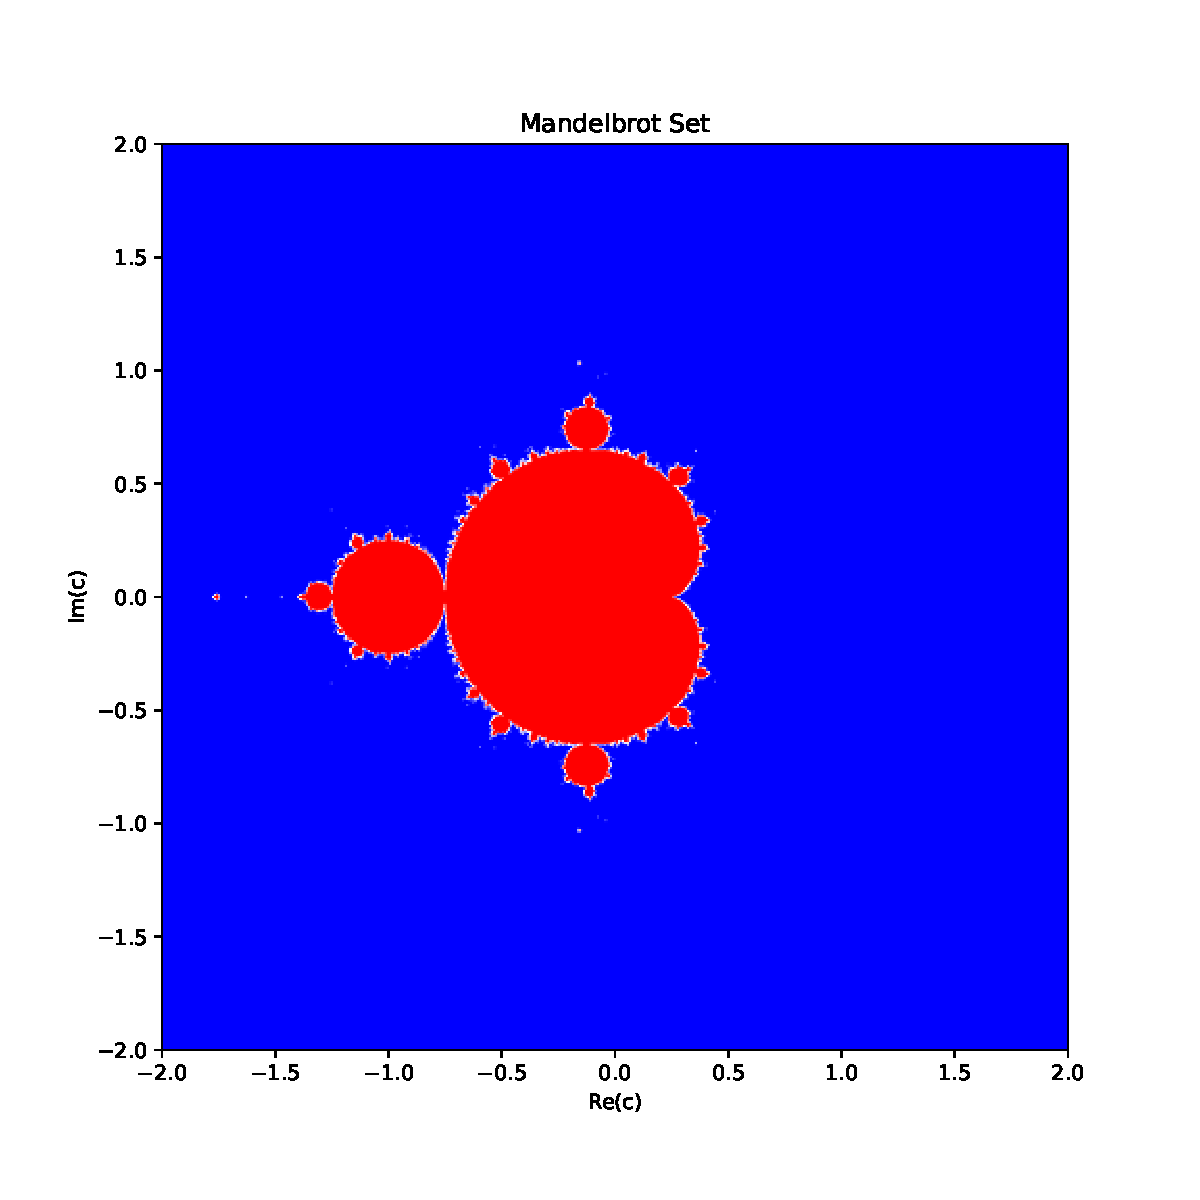
\includegraphics[width=0.7\textwidth]{q1_mandelbrot_bounded.pdf}
    \caption{Mandelbrot set: bounded points vs diverging points.}
\end{figure}

\begin{figure}[h]
    \centering
    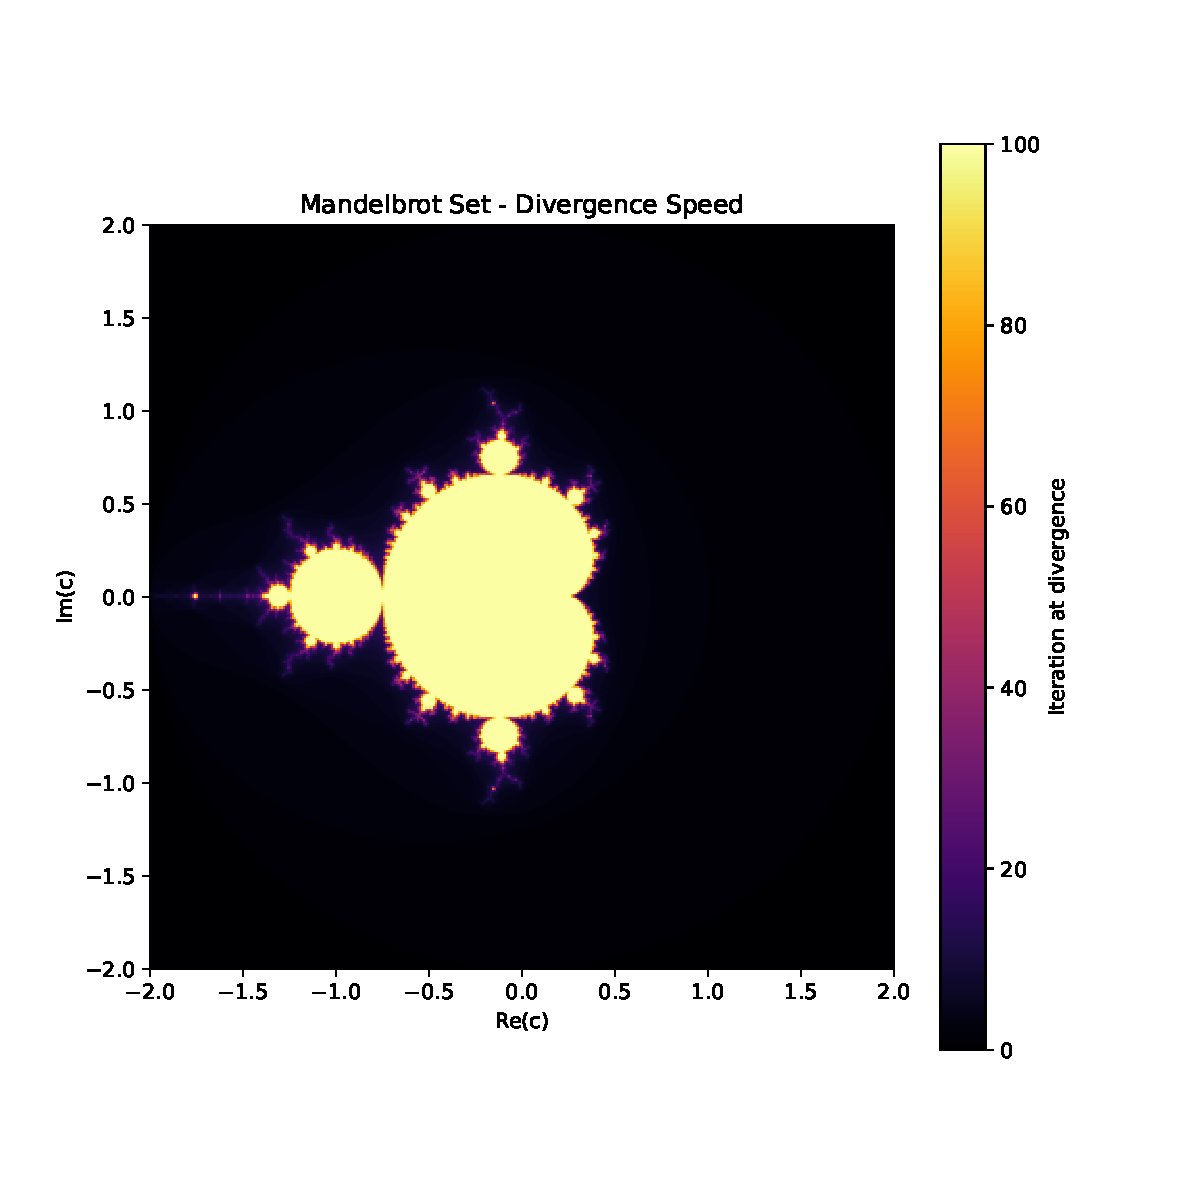
\includegraphics[width=0.7\textwidth]{q1_mandelbrot_divergence.pdf}
    \caption{Mandelbrot set colored by divergence iteration number.}
\end{figure}

\section{Question 2: The Lorenz System}

\subsection{Methods}
The Lorenz equations are a system of three coupled ordinary differential equations:
\begin{align}
\dot{X} &= -\sigma(X - Y) \\
\dot{Y} &= rX - Y - XZ \\
\dot{Z} &= -bZ + XY
\end{align}
where the parameters used are $\sigma = 10$, $r = 28$, and $b = 8/3$, with initial conditions $W_0 = [0, 1, 0]$. The equations were solved using \texttt{solve\_ivp} from \texttt{scipy.integrate} over $t = 60$ dimensionless time units with a maximum step size of $\Delta t = 0.01$.

\subsection{Results}
Figure 3 reproduces Lorenz's Figure 1, showing $Y$ as a function of iteration number $N = t/\Delta t$ over 3000 iterations. The solution shows increasingly irregular oscillations over time.

\begin{figure}[h]
    \centering
    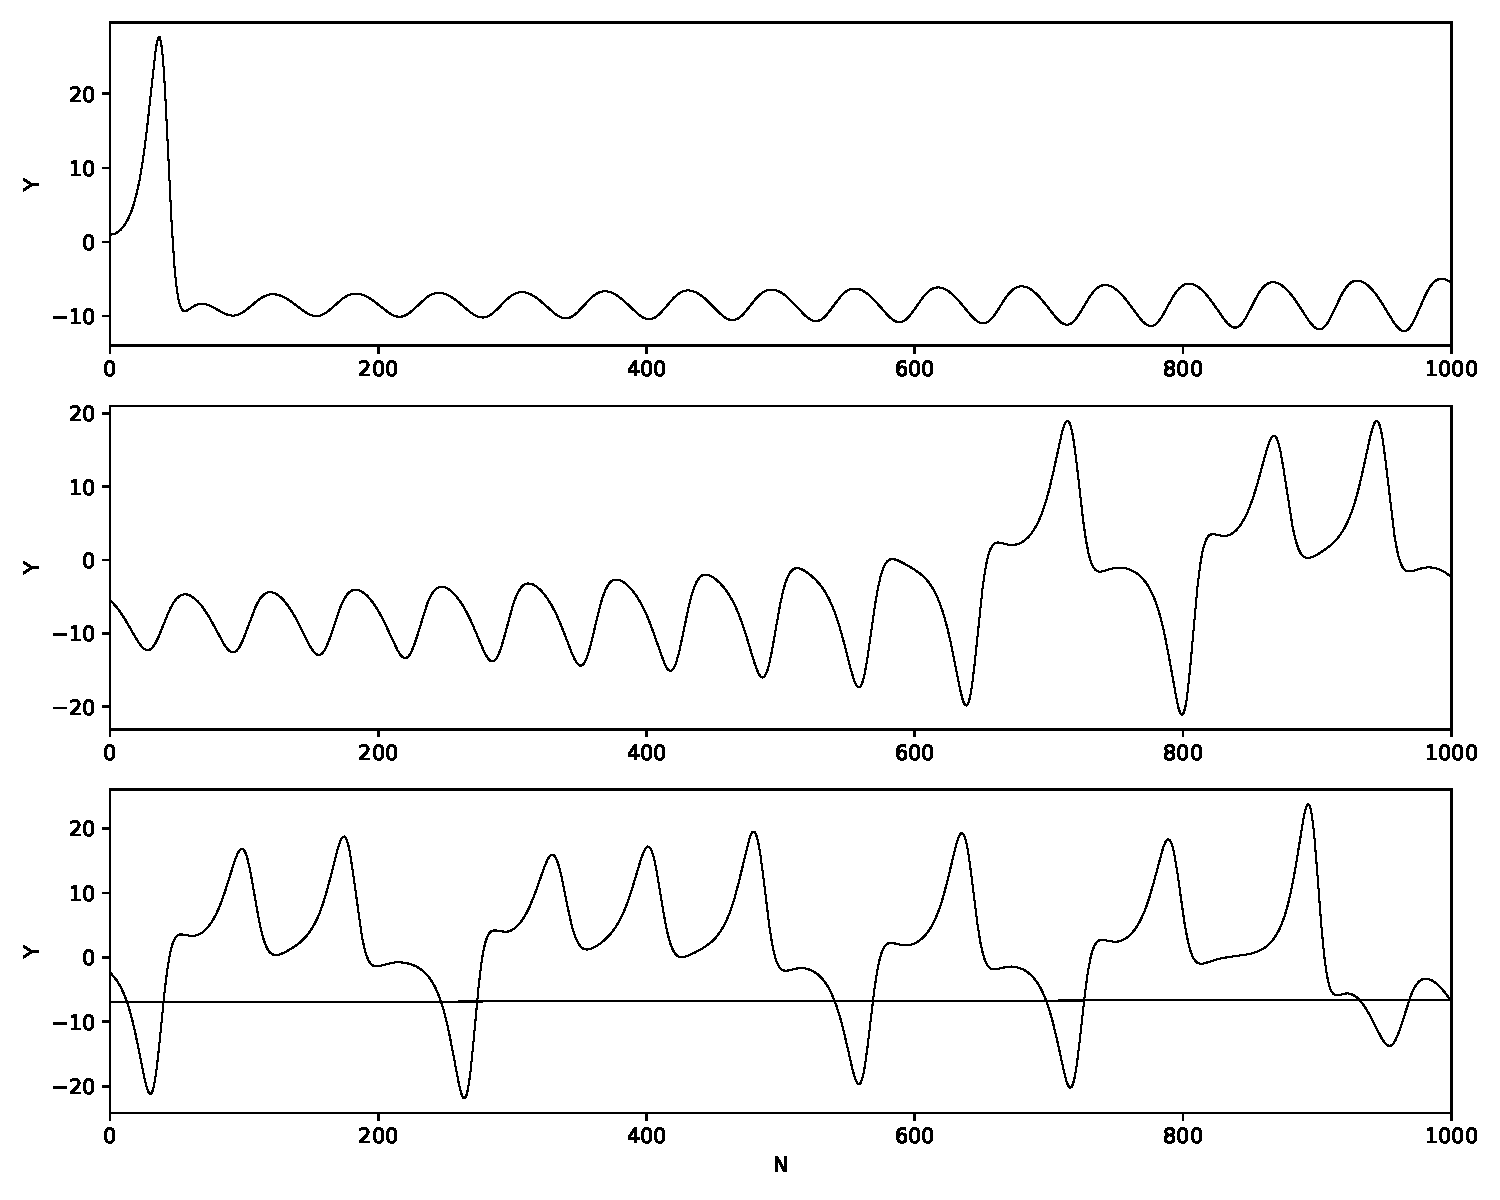
\includegraphics[width=0.7\textwidth]{q2_figure1.pdf}
    \caption{Reproduction of Lorenz Figure 1: Y vs N over 3000 iterations.}
\end{figure}

Figure 4 reproduces Lorenz's Figure 2, showing projections of the solution trajectory in the $Y$-$Z$ and $X$-$Y$ planes between iterations 1400 and 1900. The characteristic butterfly-shaped attractor is visible.

\begin{figure}[h]
    \centering
    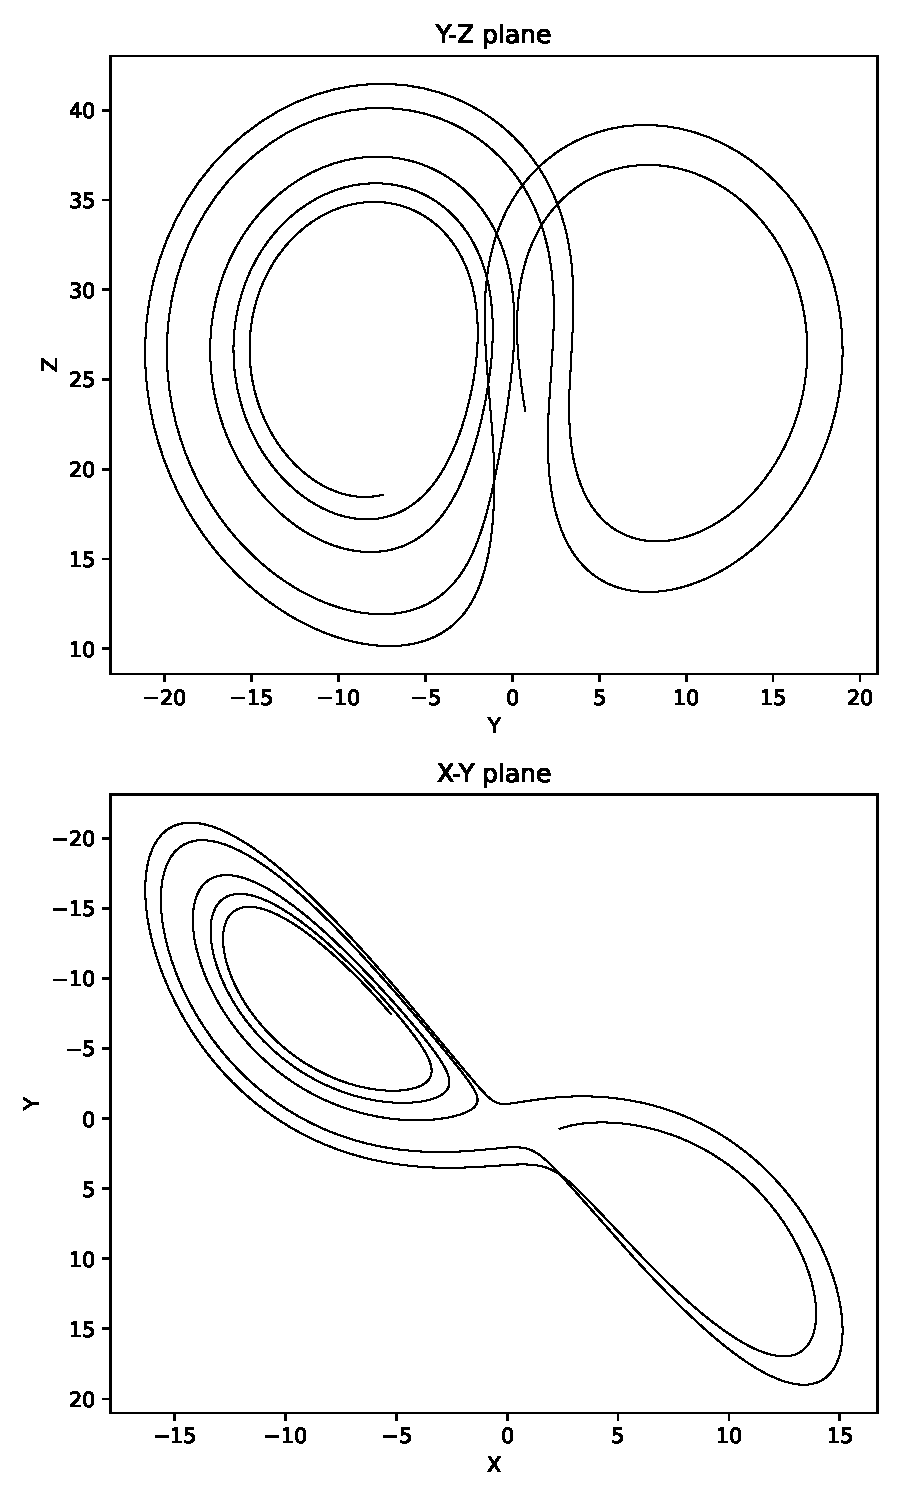
\includegraphics[width=0.7\textwidth]{q2_figure2.pdf}
    \caption{Reproduction of Lorenz Figure 2: phase space projections.}
\end{figure}

To investigate sensitivity to initial conditions, the equations were solved again with a slightly perturbed initial condition $W_0' = W_0 + [0, 10^{-8}, 0]$. The distance between the two solutions was calculated as:
\begin{equation}
d(t) = \sqrt{(X-X')^2 + (Y-Y')^2 + (Z-Z')^2}
\end{equation}

Figure 5 shows this distance on a semilog plot. The straight line up to $t \approx 30$ confirms exponential growth of the initial error, demonstrating the chaotic nature of the Lorenz system. After $t \approx 30$, the distance saturates as the solutions become completely independent.

\begin{figure}[h]
    \centering
    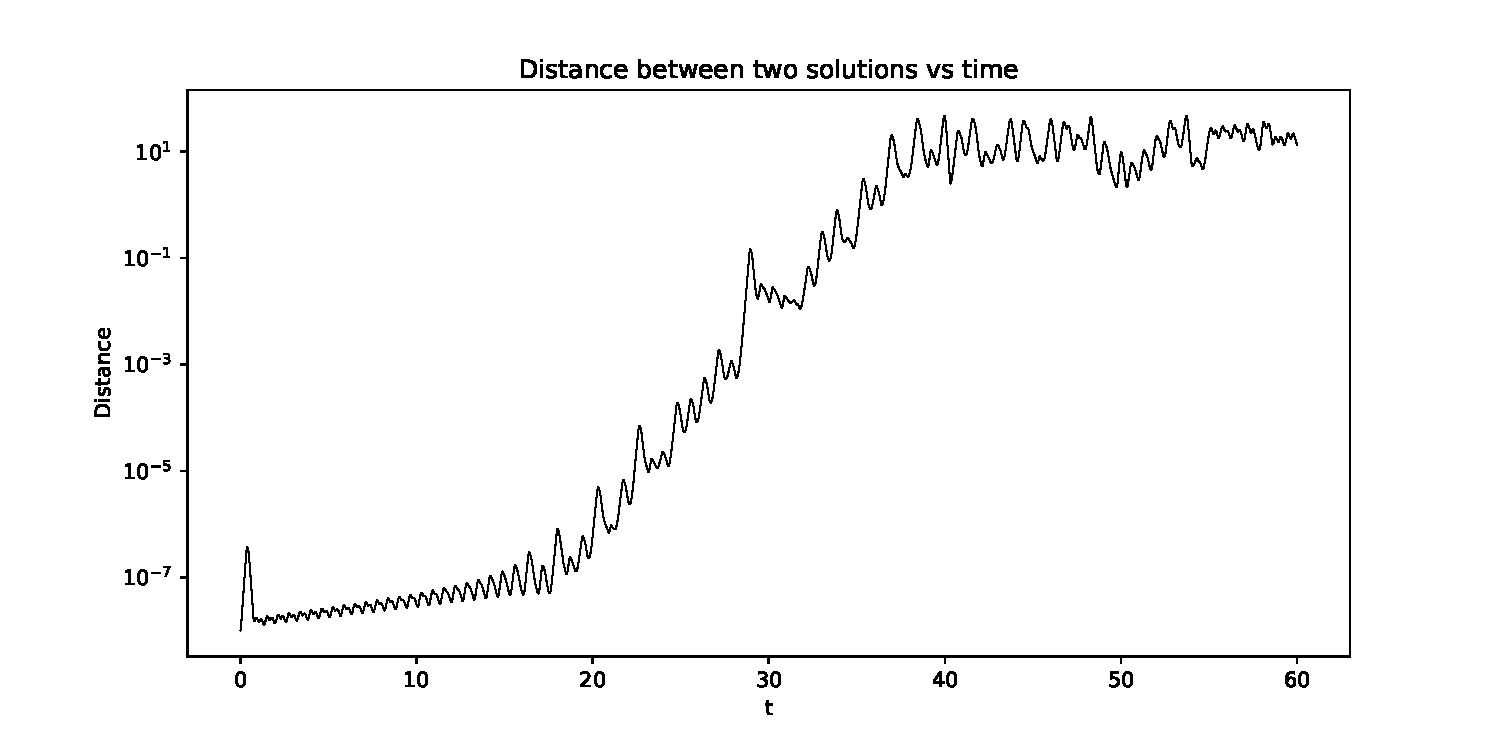
\includegraphics[width=0.7\textwidth]{q2_semilog.pdf}
    \caption{Distance between two solutions with slightly different initial conditions on a semilog plot.}
\end{figure}

\end{document}